\documentclass[
  % lualatex,
    a4paper
]{article}

% ------------------------------ font
\usepackage{times}

% ------------------------------ math
\usepackage{amsmath,amssymb}
\usepackage{siunitx}

% ------------------------------ author & natbib
\usepackage{authblk}
\usepackage[semicolon]{natbib}
\bibliographystyle{agsm}

% ------------------------------ appendix
\usepackage[title]{appendix}

% ------------------------------ tables
\usepackage{here}
\usepackage{longtable, booktabs, array}
\usepackage{threeparttable, threeparttablex, multirow}
% \newcolumntype{d}{S[input-symbols = ()]}

% ------------------------------- figures
\usepackage{graphics, graphicx}
\makeatletter
\def\maxwidth{\ifdim\Gin@nat@width>\linewidth\linewidth\else\Gin@nat@width\fi}
\def\maxheight{\ifdim\Gin@nat@height>\textheight\textheight\else\Gin@nat@height\fi}
\makeatother
% Scale images if necessary, so that they will not overflow the page
% margins by default, and it is still possible to overwrite the defaults
% using explicit options in \includegraphics[width, height, ...]{}
\setkeys{Gin}{width=\maxwidth,height=\maxheight,keepaspectratio}

% ------------------------------ page settings
\usepackage[left=3cm,right=3cm,top=3cm,bottom=3cm]{geometry}
\usepackage{setspace}
\renewcommand{\baselinestretch}{1.5}
\providecommand{\tightlist}{%
  \setlength{\itemsep}{0pt}\setlength{\parskip}{0pt}}

% ------------------------------ hyperlink
\usepackage{hyperref}

% ------------------------------ other packages
\makeatletter
\@addtoreset{table}{section}
\@addtoreset{figure}{section}
\makeatother
\renewcommand\thetable{\thesection\arabic{table}}
\renewcommand\thefigure{\thesection\arabic{figure}}
\usepackage{booktabs}
\usepackage{longtable}
\usepackage{array}
\usepackage{multirow}
\usepackage{wrapfig}
\usepackage{float}
\usepackage{colortbl}
\usepackage{pdflscape}
\usepackage{tabu}
\usepackage{threeparttable}
\usepackage{threeparttablex}
\usepackage[normalem]{ulem}
\usepackage{makecell}
\usepackage{xcolor}
\usepackage{siunitx}

  \newcolumntype{d}{S[
    input-open-uncertainty=,
    input-close-uncertainty=,
    parse-numbers = false,
    table-align-text-pre=false,
    table-align-text-post=false
  ]}
  

% ------------------------------ paper information
\title{Supplementary Material
``Adding Nudge-based Reminders to Financial Incentives for Promoting Antibody Testing and Vaccination to Prevent the Spread of Rubella''}
\author[a]{Hiroki Kato}
\author[b]{Shusaku Sasaki}
\author[b]{Fumio Ohtake}
\affil[a]{Graduate School of Economics, Osaka University}
\affil[b]{Center for Infectious Disease Education and Research (CiDER), Osaka University}
\date{}

\makeatletter
\let\@fnsymbol\@arabic
\makeatother

\begin{document}
\begin{spacing}{1}
\maketitle
\end{spacing}


{
\setcounter{tocdepth}{2}
\tableofcontents
}

\setcounter{footnote}{0}
\hypertarget{appendix-appendix}{%
\appendix}


\hypertarget{detail-background-of-rubella}{%
\section{Detail Background of Rubella}\label{detail-background-of-rubella}}

Rubella is a highly contagious disease spread through droplet transmission. The most common symptoms are fever and rashes, but the disease is rarely severe. According to the National Institute of Infectious Diseases (NIID), the subclinical transmission of rubella (the state in which a person is infected but has no symptoms) occurs in approximately 15--30\% of cases. Fever is observed in approximately 50\% of patients. Adults may also experience transient arthritis (5--30\%). Rarely, complications such as thrombocytopenic purpura (\(0.02\)--\(0.03\)\%) and acute encephalitis (\(0.01\)--\(0.03\)\%) may require hospitalization.\footnote{\url{https://www.niid.go.jp/niid/ja/kansennohanashi/430-rubella-intro.html}. Japanese. Accessed September 22, 2023.}

The most serious problem is that women infected with rubella during early pregnancy may have children with congenital rubella syndrome (CRS), which includes eye and ear defects. Because the spread of rubella tends to increase the CRS incidence, the Japanese government has designated rubella as a disease requiring immunization.

According to \citet{Kinoshita2016}, Japan can obtain herd immunity against rubella if the antibody prevalence exceeds 90\% in all generations. Some researches show relatively weak conditions to obtain herd immunity. For example, according to \citet{Plans-Rubio2012}, an antibody prevalence of 83--95\% achieves herd immunity against rubella. \citet{Nishiura2015} found that the antibody prevalence for herd immunity is 83.6\%.

Anyway, owing to low antibody prevalence among men in their 40s and 50s, Japan has not achieved herd immunity to rubella. According to \citet{NIIDdata2019}, the antibody prevalence among men aged 39--56 years (as of 2018) is approximately \(81.5\)\%. This value is lower than that of women of the same generation (about \(97.9\)\%) who have had at least one dose of the rubella vaccine administered as part of routine immunization. The prevalence rates of antibodies in men and women aged 57 and older are 91.1\% and 89.3\%, respectively. Despite not having received routine vaccination, men and women aged 57 and older grew up during a time when rubella was common and people are likely to have antibodies from natural infection. The antibody prevalence of men and women aged 38 years and younger is 91.3\% and 94.0\%, respectively. They have had at least one dose of the rubella vaccine administered as part of routine immunization.

Thus, the influx of viruses of Southeast Asian origin caused rubella epidemics in 2013 and 2018, mainly among men with relatively low antibody prevalence \citep{NIID2019}. In the 2018 epidemic, the U.S. Centers for Disease Control and Prevention advised pregnant women not to travel to Japan.\footnote{The Japan Times, October 24, 2018. \url{https://www.japantimes.co.jp/news/2018/10/24/national/science-health/u-s-cdc-warns-pregnant-women-traveling-japan-amid-rubella-outbreak/}. Accessed September 22, 2023.} As cross-border traffic is increasing, achieving herd immunity against rubella is becoming increasingly important for Japan.

To achieve herd immunity, Japan must raise the antibody prevalence among men in their 40s and 50s from 80\% to 90\%. To achieve this goal, The Ministry of Health, Labour and Welfare (MHLW) provided the rubella antibody test and vaccination as an additional free routine immunization for men aged 40--57 years (as of 2019) between April 2019 and March 2022. More precisely, eligible men were born between April 2, 1962 and April 1, 1979.

If transmission to pregnant women is the most important issue, one might think that vaccinating pregnant women would be the optimal strategy. However, Japan implemented measures for pregnant women in advance of the 2019 vaccination campaign, as they were already receiving at least one vaccination. In addition, since 2014, pregnant women and women who want to become pregnant as well as their partners have been offered free antibody testing. However, during the 2013 and 2018 epidemics, some infants were affected by CRS. Therefore, to eradicate CRS, interventions for pregnant women alone are insufficient; interventions to achieve hard immunity are needed.

The MHLW requested local governments to send free vouchers for a rubella antibody test and vaccine to eligible men over a three-year period. More than half of eligible men are 40--46 years old (\(6.46\) million). They received the free vouchers from April 2019 to March 2020. According to interviews conducted by the MHLW, approximately 96\% of local governments planned to send the vouchers by October 2019. The cumulative number of antibody tests using vouchers by January 2019 was 1.17 million. We calculate the actual uptake of antibody testing by dividing the cumulative number of antibody tests using vouchers to January 2020 (\(1.17\) million) by the population of 40--46-year-old men (\(6.46\) million). Thus, although men aged 40--46 years automatically received the financial incentives, the actual uptake of antibody testing with vouchers remained as low as 18\% as of January 2020. When the financial incentives offered are adequate, as in the presented case, non-monetary interventions should be considered to increase antibody testing.

\clearpage

\hypertarget{question}{%
\section{Antibody Testing and Vaccination Questions}\label{question}}

In Wave 2, the participants were asked if they had undertaken antibody testing and been vaccinated since Wave 1. The antibody testing question asked, ``Have you undertaken rubella antibody testing since the end of the last survey?'' The participants were given the following choices:

\begin{itemize}
\item
  \begin{enumerate}
  \def\labelenumi{(\alph{enumi})}
  \tightlist
  \item
    Yes, I have undertaken antibody testing;
  \end{enumerate}
\item
  \begin{enumerate}
  \def\labelenumi{(\alph{enumi})}
  \setcounter{enumi}{1}
  \tightlist
  \item
    No, I have not undertaken antibody testing;
  \end{enumerate}
\item
  \begin{enumerate}
  \def\labelenumi{(\alph{enumi})}
  \setcounter{enumi}{2}
  \tightlist
  \item
    I underwent antibody testing before the last survey.
  \end{enumerate}
\end{itemize}

We created a binary variable coded 1 if the respondent chose option (a) and used it as an outcome variable for the actual uptake of antibody testing. Meanwhile, the vaccination question was ``Have you been vaccinated against rubella since the end of the last survey?'' The respondents were given five options:

\begin{itemize}
\item
  \begin{enumerate}
  \def\labelenumi{(\alph{enumi})}
  \tightlist
  \item
    I have been vaccinated;
  \end{enumerate}
\item
  \begin{enumerate}
  \def\labelenumi{(\alph{enumi})}
  \setcounter{enumi}{1}
  \tightlist
  \item
    I do not need the vaccine due to a positive test or infection experience;
  \end{enumerate}
\item
  \begin{enumerate}
  \def\labelenumi{(\alph{enumi})}
  \setcounter{enumi}{2}
  \tightlist
  \item
    I have undertaken antibody testing but have not been vaccinated yet;
  \end{enumerate}
\item
  \begin{enumerate}
  \def\labelenumi{(\alph{enumi})}
  \setcounter{enumi}{3}
  \tightlist
  \item
    I have not undertaken antibody testing or gotten vaccinated;
  \end{enumerate}
\item
  \begin{enumerate}
  \def\labelenumi{(\alph{enumi})}
  \setcounter{enumi}{4}
  \tightlist
  \item
    I was vaccinated before the last survey.
  \end{enumerate}
\end{itemize}

We created a binary variable coded 1 if the participant chose option (a) for both the antibody testing and the vaccination questions. Then, we used it as the outcome variable for vaccination rates.

\clearpage

\hypertarget{method-value}{%
\section{Estimation of the Monetary Value of the Text Message Reminders}\label{method-value}}

To determine the extent to which the text message reminders increase the monetary value of the rubella vaccination, we use the WTP for the vaccination. Let \(WTP_i\) be an individual's WTP that follows a cumulative distribution \(F\). Then, for a given cost \(C\), men will be vaccinated if \(WTP_i \ge C\). The vaccination rate is \(F_0 = 1-F(C)\). Suppose that our treated text message reminders change the WTP by \(\beta\). An individual who receives a treated text message reminder will be vaccinated if \(WTP_i\ge C-\beta\). The vaccination rate of the treated group is \(F_1 = 1-F(C-\beta)\). Thus, the treatment effect is \(\tau = F_1-F_0=F(C)-F(C-\beta)\). From the perspective of government subsidies, the subsidy equal to the effect of the text message reminder \(\tau\) is \(\beta\). We want to estimate \(\beta\).

\begin{figure}[t]
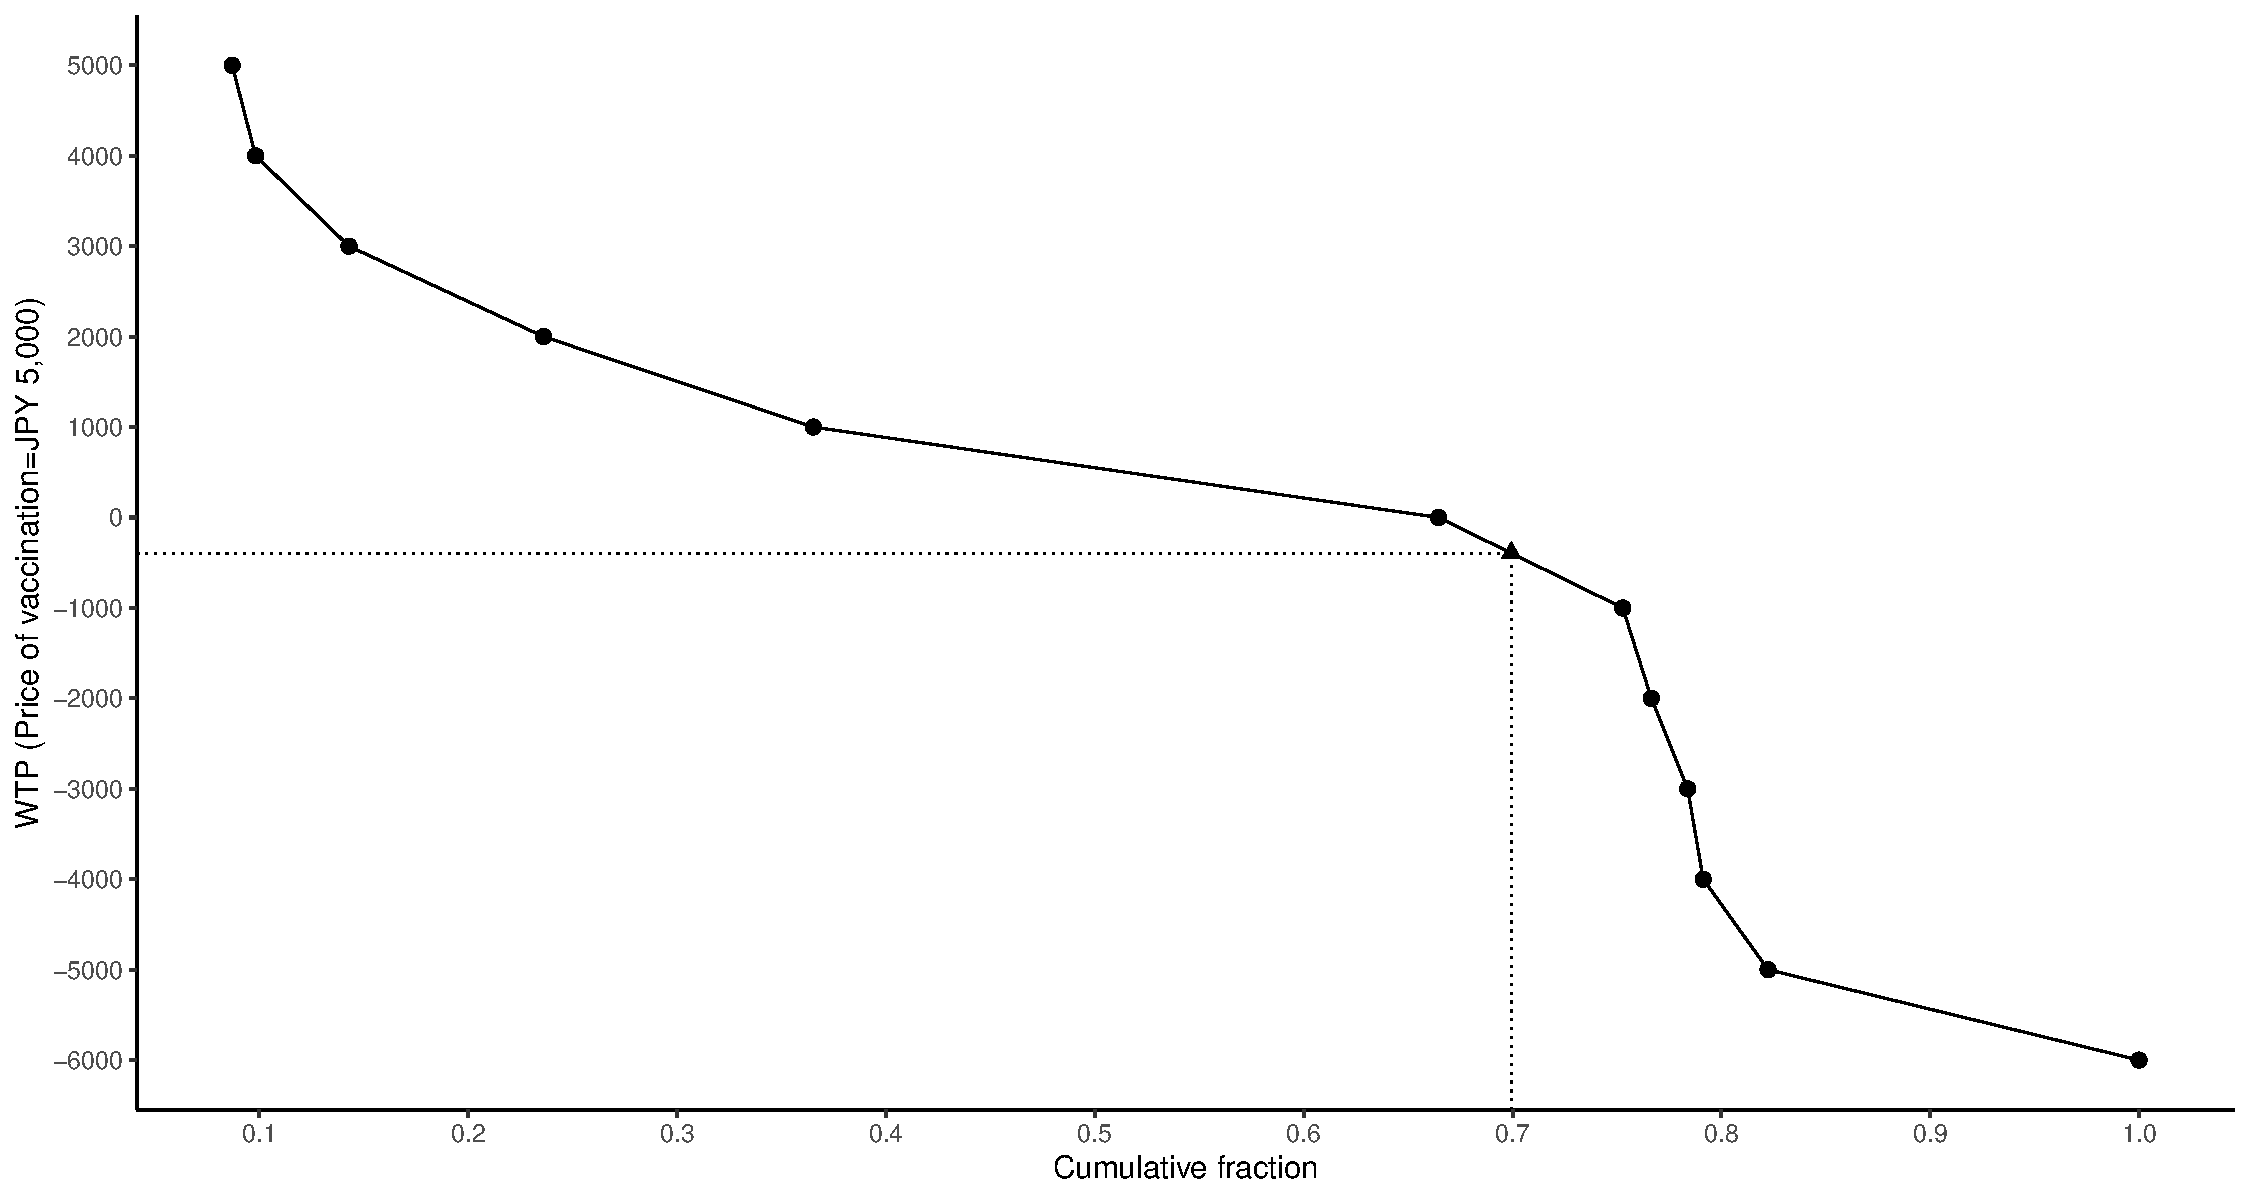
\includegraphics{Supplementary-Material_files/figure-latex/demand-function-1} \caption{Demand Curve of the Rubella Vaccination for the \emph{Default Incentive} Group. Notes: Black triangles indicate the baseline vaccination rate $F_0$ and corresponding WTP.}\label{fig:demand-function}
\end{figure}

Once \(F\), \(C\), and \(\tau\) are determined, we obtain \(\beta\). We first discuss the estimation of \(F\) (demand function). We elicit the WTP for the vaccination in Wave 1 before the participants read their message. If the vaccination costs JPY 5,000, we ask the respondents if they would be vaccinated if the local government pays \(s_j\). The subsidy amounts are \(s_j \in \{0, 1000, 2000, \ldots , 10000\}\). Let \(s_i^{\text{min}}\) be the lowest subsidy at which the respondents indicate that they would be vaccinated. Let \(s_i^{\text{max}}\) be the highest subsidy that the respondents indicate they would not be vaccinated. We can identify the WTP for the vaccination within the range \([5000 - s_i^{\text{max}}, 5000 - s_i^{\text{min}})\). Thus, without additional assumptions, the demand curve is step-wise, and we estimate the monetary value of the effect of the text message reminders with bounds. If the respondents indicate that they would not be vaccinated at all the subsidy amounts, then \(s_i^{\text{max}} = 10000\). However, we cannot define \(s_i^{\text{min}}\) in the data. Therefore, we assume \(s_i^{\text{min}} = 11000\). This assumption does not affect the monetary value of the text message reminders. To obtain a point estimate, we assume that the true WTP is uniformly distributed within the range \([5000 - s_i^{\text{max}}, 5000 - s_i^{\text{min}})\). The vaccination demand curve can then be linearly interpolated (see Figure \ref{fig:demand-function}).

In the \emph{default incentive} group, eligible men receive a free vaccination. Therefore, the natural setting is \(C=0\). In addition, we use the effect on the actual uptake of antibody testing as the effect of the text message reminders \(\tau\). The person taking the antibody test wants to obtain the antibody against rubella. However, the effect of the text message reminder on vaccination rates differs from the effect on the (true) intention to be vaccinated because people with a positive antibody test result cannot be vaccinated. Therefore, \(\tau\) is the effect on antibody testing rather than on vaccination rates.

In our framework, \(F_0=1-F(0)\), but one potential concern remains. The effect of the text message reminders \(\tau\) is estimated as the difference from the MHLW (Control) group. Assuming that everyone who did not participate in our survey did not take the antibody test after the survey, the actual uptake of antibody testing of MHLW (Control) can be considered as an effect of providing the message in the survey. To remove this effect, we instead use \(F_0=(1-F(0))+(F(0)-F(-\alpha))\). The second term is the antibody testing rate of the control group (\(3.5\)\%) under no vaccination cost. The demand function is estimated to be \(F_0=0.7\) and \(\alpha=394\). Finally, we find \(\beta\) holding that \(\tau=F(-\alpha)-F(-\beta)\).

\clearpage

\hypertarget{fig-tab}{%
\section{Tables}\label{fig-tab}}

\begin{table}[!h]

\caption{\label{tab:covariate-list}List of the Covariates}
\centering
\fontsize{9}{11}\selectfont
\begin{tabular}[t]{l>{\raggedright\arraybackslash}p{30em}cc}
\toprule
  & Description & Mean & Std.Dev.\\
\midrule
age & (Wave1) Age as of April 2019 based on year of birth and month of birth. & \num{48.66} & \num{5.69}\\
married & (Wave1) Dummy variable taking one if a respondent is married. & \num{0.58} & \num{0.49}\\
education & (Wave1) Years of education. & \num{14.75} & \num{2.31}\\
income & (Wave1) Household income. For those who did not respond with household income, the overall average was used. & \num{684.90} & \num{375.74}\\
noinfo\_income & (Wave1) Dummy variable taking one if a respondent did not answer household income. & \num{0.15} & \num{0.36}\\
exercise\_w1 & (Wave1) Dummy variable taking one if a respondent exercises or plays sports more than once a week. & \num{0.22} & \num{0.42}\\
health\_check & (Wave1) Dummy variable taking one if a respondent has had a medical examination in their city or place of employment in the past year from the time of Wave 1. & \num{0.68} & \num{0.46}\\
flushot & (Wave1) Dummy variable taking one if a respondent is vaccinated against influenza every year. & \num{0.27} & \num{0.45}\\
norm\_waiting\_line & (Wave1) Five-point Likert scale for the question "I never interrupt someone in line." & \num{4.07} & \num{0.96}\\
selfish\_anonymous & (Wave1) Five-point Likert scale for the question "If I can never find it, I can do bad things (littering, parking tickets, etc.)." & \num{2.33} & \num{0.98}\\
handwash & (Wave2) Five-point Likert scale for the question "I washed my hands and gargled frequently from the end of the previous survey to today." & \num{3.91} & \num{1.04}\\
temp\_check & (Wave2) Five-point Likert scale for the question "I took my temperature frequently from the end of the previous survey to today." & \num{2.26} & \num{1.22}\\
avoid\_out & (Wave2) Five-point Likert scale for the question "I refrained from going out from the end of the previous survey to today." & \num{2.96} & \num{1.20}\\
avoid\_crowd & (Wave2) Five-point Likert scale for the question "I avoided crowded places when I went out from the end of the previous survey to today." & \num{3.38} & \num{1.10}\\
wear\_mask & (Wave2) Five-point Likert scale for the question "I always wore a medical mask when I went out or met people from the end of the previous survey to today." & \num{3.14} & \num{1.38}\\
\bottomrule
\end{tabular}
\end{table}

\begin{table}[!h]

\caption{\label{tab:balance-int-default}Balance Tests for the \emph{Default Incentive} Group (Sample for Estimating the Effect on Intention)}
\centering
\fontsize{9}{11}\selectfont
\begin{threeparttable}
\begin{tabular}[t]{l>{\centering\arraybackslash}p{3em}>{\centering\arraybackslash}p{3em}>{\centering\arraybackslash}p{3em}>{\centering\arraybackslash}p{3em}>{\centering\arraybackslash}p{3em}>{\centering\arraybackslash}p{3em}>{\centering\arraybackslash}p{3em}c}
\toprule
 & MHLW (Control) & MHLW (Age) & Altruistic & Selfish & Social Comparison & Deadline & Convenient & F-test, p-value\\
\midrule
age & 42.862 & 43.046 & 43.135 & 43.045 & 42.909 & 42.906 & 42.866 & 0.874\\
married & 0.408 & 0.458 & 0.412 & 0.417 & 0.455 & 0.478 & 0.480 & 0.785\\
education & 14.654 & 14.473 & 14.595 & 14.205 & 14.099 & 14.348 & 14.575 & 0.446\\
income & 557.562 & 645.556 & 613.156 & 623.542 & 569.530 & 590.422 & 633.487 & 0.149\\
noinfo\_income & 0.162 & 0.168 & 0.203 & 0.197 & 0.157 & 0.130 & 0.181 & 0.706\\
exercise\_w1 & 0.246 & 0.176 & 0.277 & 0.189 & 0.165 & 0.217 & 0.213 & 0.285\\
health\_check & 0.654 & 0.626 & 0.696 & 0.538 & 0.603 & 0.674 & 0.614 & 0.150\\
flushot & 0.238 & 0.260 & 0.203 & 0.144 & 0.140 & 0.239 & 0.236 & 0.055\\
norm\_waiting\_line & 4.100 & 3.908 & 3.892 & 3.970 & 4.050 & 3.906 & 4.024 & 0.447\\
selfish\_anonymous & 2.377 & 2.435 & 2.331 & 2.371 & 2.446 & 2.355 & 2.425 & 0.945\\
\bottomrule
\end{tabular}
\begin{tablenotes}
\item Notes: Table \ref{tab:covariate-list} describes the variables. Columns (2)--(8) show the sample averages for each experimental arm. Column (9) shows the p-value of the joint null hypothesis (F-test).
\end{tablenotes}
\end{threeparttable}
\end{table}

\begin{table}[!h]

\caption{\label{tab:balance-int-optin}Balance Tests for the \emph{Opt-In Incentive} Group (Sample for Estimating the Effect on Intention)}
\centering
\fontsize{9}{11}\selectfont
\begin{threeparttable}
\begin{tabular}[t]{l>{\centering\arraybackslash}p{3em}>{\centering\arraybackslash}p{3em}>{\centering\arraybackslash}p{3em}>{\centering\arraybackslash}p{3em}>{\centering\arraybackslash}p{3em}>{\centering\arraybackslash}p{3em}>{\centering\arraybackslash}p{3em}c}
\toprule
 & MHLW (Control) & MHLW (Age) & Altruistic & Selfish & Social Comparison & Deadline & Convenient & F-test, p-value\\
\midrule
age & 51.632 & 51.408 & 51.226 & 51.657 & 51.582 & 51.545 & 51.502 & 0.712\\
married & 0.600 & 0.588 & 0.628 & 0.657 & 0.602 & 0.549 & 0.619 & 0.334\\
education & 14.572 & 14.655 & 14.530 & 14.830 & 14.566 & 14.634 & 14.393 & 0.578\\
income & 712.622 & 707.190 & 687.764 & 677.141 & 656.419 & 707.708 & 710.713 & 0.540\\
noinfo\_income & 0.184 & 0.164 & 0.145 & 0.117 & 0.155 & 0.163 & 0.205 & 0.211\\
exercise\_w1 & 0.156 & 0.193 & 0.239 & 0.230 & 0.183 & 0.203 & 0.218 & 0.252\\
health\_check & 0.632 & 0.664 & 0.701 & 0.683 & 0.653 & 0.659 & 0.644 & 0.742\\
flushot & 0.228 & 0.244 & 0.197 & 0.270 & 0.275 & 0.228 & 0.251 & 0.433\\
norm\_waiting\_line & 4.136 & 4.134 & 4.137 & 4.078 & 4.004 & 4.028 & 4.063 & 0.590\\
selfish\_anonymous & 2.416 & 2.231 & 2.325 & 2.374 & 2.223 & 2.337 & 2.368 & 0.201\\
\bottomrule
\end{tabular}
\begin{tablenotes}
\item Notes: Table \ref{tab:covariate-list} describes the variables. Columns (2)--(8) show the sample averages for each experimental arm. Column (9) shows the p-value of the joint null hypothesis (F-test).
\end{tablenotes}
\end{threeparttable}
\end{table}

\begin{table}

\caption{\label{tab:diff-in-mean-int}Difference-in-means Test of Intention}
\centering
\fontsize{9}{11}\selectfont
\begin{threeparttable}
\begin{tabular}[t]{lcccccc}
\toprule
\multicolumn{1}{c}{ } & \multicolumn{3}{c}{Antibody testing} & \multicolumn{3}{c}{Vaccination} \\
\cmidrule(l{3pt}r{3pt}){2-4} \cmidrule(l{3pt}r{3pt}){5-7}
\multicolumn{2}{c}{ } & \multicolumn{2}{c}{P-values} & \multicolumn{1}{c}{ } & \multicolumn{2}{c}{P-values} \\
\cmidrule(l{3pt}r{3pt}){3-4} \cmidrule(l{3pt}r{3pt}){6-7}
Treatment & Effect & T-test & Exact test & Effect & T-test & Exact test\\
\midrule
\addlinespace[0.3em]
\multicolumn{7}{l}{\textbf{A. Default incentive group}}\\
\hspace{1em}MHLW (Age) & 2.132 & 0.678 & 0.775 & 1.973 & 0.748 & 0.825\\
\hspace{1em}Altruistic & 14.366 & 0.007 & 0.005 & 2.380 & 0.690 & 0.720\\
\hspace{1em}Selfish & 7.261 & 0.172 & 0.210 & 3.916 & 0.524 & 0.540\\
\hspace{1em}Social Comparison & 4.024 & 0.450 & 0.485 & 1.437 & 0.819 & 0.920\\
\hspace{1em}Deadline & 3.144 & 0.538 & 0.545 & -0.959 & 0.874 & 0.890\\
\hspace{1em}Convenient & 5.215 & 0.325 & 0.425 & 1.769 & 0.775 & 0.800\\
\addlinespace[0.3em]
\multicolumn{7}{l}{\textbf{B. Opt-in incentive group}}\\
\hspace{1em}MHLW (Age) & -2.390 & 0.550 & 0.605 & -6.582 & 0.147 & 0.145\\
\hspace{1em}Altruistic & 5.306 & 0.205 & 0.190 & -2.800 & 0.539 & 0.570\\
\hspace{1em}Selfish & 4.139 & 0.323 & 0.380 & -2.800 & 0.541 & 0.585\\
\hspace{1em}Social Comparison & -3.696 & 0.345 & 0.400 & -8.178 & 0.067 & 0.085\\
\hspace{1em}Deadline & 2.888 & 0.480 & 0.430 & -2.800 & 0.534 & 0.560\\
\hspace{1em}Convenient & 6.291 & 0.133 & 0.180 & -3.009 & 0.507 & 0.510\\
\bottomrule
\end{tabular}
\begin{tablenotes}
\item Notes: The unit of effect is a percentage point. Fisher's exact p-values test sharp null hypotheses. To calculate p-values, we create 200 simulated assignment vector keeping the number of treated and contrl units fixed.
\end{tablenotes}
\end{threeparttable}
\end{table}

\begin{table}[!h]

\caption{\label{tab:balance-act-default}Balance Tests for the \emph{Default Incentive} group (Sample for Estimating the Effect on Behavior)}
\centering
\fontsize{9}{11}\selectfont
\begin{threeparttable}
\begin{tabular}[t]{l>{\centering\arraybackslash}p{3em}>{\centering\arraybackslash}p{3em}>{\centering\arraybackslash}p{3em}>{\centering\arraybackslash}p{3em}>{\centering\arraybackslash}p{3em}>{\centering\arraybackslash}p{3em}>{\centering\arraybackslash}p{3em}c}
\toprule
 & MHLW (Control) & MHLW (Age) & Altruistic & Selfish & Social Comparison & Deadline & Convenient & F-test, p-value\\
\midrule
age & 42.861 & 43.059 & 43.102 & 43.036 & 42.893 & 42.898 & 42.964 & 0.953\\
married & 0.391 & 0.454 & 0.391 & 0.360 & 0.437 & 0.466 & 0.477 & 0.467\\
education & 14.496 & 14.471 & 14.547 & 14.126 & 14.010 & 14.407 & 14.595 & 0.474\\
income & 548.244 & 649.778 & 614.512 & 599.124 & 555.083 & 591.597 & 637.056 & 0.102\\
noinfo\_income & 0.174 & 0.126 & 0.203 & 0.207 & 0.146 & 0.136 & 0.171 & 0.522\\
exercise\_w1 & 0.252 & 0.185 & 0.266 & 0.171 & 0.165 & 0.195 & 0.225 & 0.375\\
health\_check & 0.643 & 0.639 & 0.680 & 0.532 & 0.631 & 0.661 & 0.640 & 0.391\\
flushot & 0.235 & 0.261 & 0.227 & 0.135 & 0.146 & 0.246 & 0.207 & 0.082\\
norm\_waiting\_line & 4.174 & 3.933 & 3.922 & 4.036 & 4.078 & 3.898 & 4.063 & 0.219\\
selfish\_anonymous & 2.339 & 2.412 & 2.367 & 2.333 & 2.447 & 2.373 & 2.414 & 0.977\\
handwash & 3.861 & 3.916 & 3.797 & 3.757 & 3.767 & 3.915 & 3.829 & 0.835\\
temp\_check & 2.139 & 2.235 & 2.414 & 2.126 & 2.204 & 2.203 & 2.117 & 0.535\\
avoid\_out & 3.096 & 3.034 & 3.047 & 2.793 & 2.932 & 3.025 & 2.928 & 0.544\\
avoid\_crowd & 3.296 & 3.336 & 3.273 & 3.234 & 3.350 & 3.305 & 3.324 & 0.990\\
wear\_mask & 2.930 & 3.076 & 3.109 & 3.009 & 3.010 & 3.144 & 3.207 & 0.794\\
\bottomrule
\end{tabular}
\begin{tablenotes}
\item Notes: Table \ref{tab:covariate-list} describes the variables. Columns (2)--(8) show the sample averages for each experimental arm. Column (9) shows the p-value of the joint null hypothesis (F-test).
\end{tablenotes}
\end{threeparttable}
\end{table}

\begin{table}[!h]

\caption{\label{tab:balance-act-optin}Balance Tests for the \emph{Opt-in Incentive} Group (Sample for Estimating the Effect on Behavior)}
\centering
\fontsize{9}{11}\selectfont
\begin{threeparttable}
\begin{tabular}[t]{l>{\centering\arraybackslash}p{3em}>{\centering\arraybackslash}p{3em}>{\centering\arraybackslash}p{3em}>{\centering\arraybackslash}p{3em}>{\centering\arraybackslash}p{3em}>{\centering\arraybackslash}p{3em}>{\centering\arraybackslash}p{3em}c}
\toprule
 & MHLW (Control) & MHLW (Age) & Altruistic & Selfish & Social Comparison & Deadline & Convenient & F-test, p-value\\
\midrule
age & 51.695 & 51.394 & 51.179 & 51.662 & 51.421 & 51.605 & 51.512 & 0.564\\
married & 0.591 & 0.560 & 0.611 & 0.652 & 0.598 & 0.547 & 0.596 & 0.407\\
education & 14.505 & 14.620 & 14.553 & 14.876 & 14.593 & 14.610 & 14.345 & 0.472\\
income & 712.165 & 707.809 & 686.355 & 671.407 & 644.798 & 699.289 & 718.575 & 0.370\\
noinfo\_income & 0.173 & 0.157 & 0.137 & 0.114 & 0.159 & 0.166 & 0.222 & 0.142\\
exercise\_w1 & 0.159 & 0.194 & 0.232 & 0.229 & 0.173 & 0.211 & 0.202 & 0.432\\
health\_check & 0.632 & 0.667 & 0.684 & 0.677 & 0.645 & 0.673 & 0.631 & 0.849\\
flushot & 0.223 & 0.245 & 0.189 & 0.264 & 0.280 & 0.215 & 0.241 & 0.376\\
norm\_waiting\_line & 4.159 & 4.162 & 4.126 & 4.065 & 3.991 & 4.063 & 4.030 & 0.431\\
selfish\_anonymous & 2.436 & 2.227 & 2.311 & 2.343 & 2.234 & 2.300 & 2.379 & 0.240\\
handwash & 3.823 & 3.889 & 3.926 & 3.751 & 3.836 & 3.861 & 3.867 & 0.769\\
temp\_check & 2.095 & 2.204 & 2.221 & 2.100 & 2.136 & 2.085 & 2.182 & 0.841\\
avoid\_out & 2.886 & 2.889 & 2.932 & 2.866 & 2.855 & 2.964 & 2.941 & 0.960\\
avoid\_crowd & 3.295 & 3.361 & 3.447 & 3.239 & 3.313 & 3.309 & 3.433 & 0.437\\
wear\_mask & 3.082 & 3.176 & 3.116 & 3.144 & 2.977 & 2.942 & 3.010 & 0.533\\
\bottomrule
\end{tabular}
\begin{tablenotes}
\item Notes: Table \ref{tab:covariate-list} describes the variables. Columns (2)--(8) show the sample averages for each experimental arm. Column (9) shows the p-value of the joint null hypothesis (F-test).
\end{tablenotes}
\end{threeparttable}
\end{table}

\begin{table}

\caption{\label{tab:diff-in-mean-act}Difference-in-means Test of Behavior}
\centering
\fontsize{9}{11}\selectfont
\begin{threeparttable}
\begin{tabular}[t]{lcccccc}
\toprule
\multicolumn{1}{c}{ } & \multicolumn{3}{c}{Antibody testing} & \multicolumn{3}{c}{Vaccination} \\
\cmidrule(l{3pt}r{3pt}){2-4} \cmidrule(l{3pt}r{3pt}){5-7}
\multicolumn{2}{c}{ } & \multicolumn{2}{c}{P-values} & \multicolumn{1}{c}{ } & \multicolumn{2}{c}{P-values} \\
\cmidrule(l{3pt}r{3pt}){3-4} \cmidrule(l{3pt}r{3pt}){6-7}
Treatment & Effect & T-test & Exact test & Effect & T-test & Exact test\\
\midrule
\addlinespace[0.3em]
\multicolumn{7}{l}{\textbf{A. Default incentive group}}\\
\hspace{1em}MHLW (Age) & 3.244 & 0.260 & 0.385 & 0.811 & 0.581 & 1.000\\
\hspace{1em}Altruistic & 7.459 & 0.023 & 0.030 & 3.818 & 0.066 & 0.115\\
\hspace{1em}Selfish & 5.531 & 0.088 & 0.115 & 1.833 & 0.303 & 0.420\\
\hspace{1em}Social Comparison & 5.260 & 0.111 & 0.170 & 3.985 & 0.085 & 0.135\\
\hspace{1em}Deadline & 0.759 & 0.765 & 1.000 & -0.022 & 0.985 & 1.000\\
\hspace{1em}Convenient & 3.729 & 0.216 & 0.295 & 1.833 & 0.303 & 0.380\\
\addlinespace[0.3em]
\multicolumn{7}{l}{\textbf{B. Opt-in incentive group}}\\
\hspace{1em}MHLW (Age) & 0.471 & 0.554 & 0.615 & 0.463 & 0.318 & 0.530\\
\hspace{1em}Altruistic & 1.651 & 0.148 & 0.200 & 0.526 & 0.319 & 0.460\\
\hspace{1em}Selfish & 1.038 & 0.286 & 0.390 & 0.498 & 0.319 & 0.475\\
\hspace{1em}Social Comparison & 2.349 & 0.055 & 0.080 & 0.000 &  & 1.000\\
\hspace{1em}Deadline & 0.891 & 0.321 & 0.695 & 0.448 & 0.318 & 1.000\\
\hspace{1em}Convenient & 0.531 & 0.523 & 0.640 & 0.000 &  & 1.000\\
\bottomrule
\end{tabular}
\begin{tablenotes}
\item Notes: The unit of effect is a percentage point. Fisher's exact p-values test sharp null hypotheses. To calculate p-values, we create 200 simulated assignment vector keeping the number of treated and contrl units fixed.
\end{tablenotes}
\end{threeparttable}
\end{table}

\begin{table}

\caption{\label{tab:reg-int-woA}Effect of the Message Content on Intention Compared with MHLW (Age)}
\centering
\fontsize{9}{11}\selectfont
\begin{threeparttable}
\begin{tabular}[t]{lcccc}
\toprule
\multicolumn{1}{c}{ } & \multicolumn{2}{c}{Testing} & \multicolumn{2}{c}{Vaccination} \\
\cmidrule(l{3pt}r{3pt}){2-3} \cmidrule(l{3pt}r{3pt}){4-5}
  & (1) & (2) & (3) & (4)\\
\midrule
Altruistic & \num{0.122} (\num{0.054}) & \num{0.124} (\num{0.051}) & \num{0.004} (\num{0.060}) & \num{-0.001} (\num{0.057})\\
 & {}[\num{0.023}] & {}[\num{0.016}] & {}[\num{0.946}] & {}[\num{0.990}]\\
Selfish & \num{0.051} (\num{0.054}) & \num{0.077} (\num{0.051}) & \num{0.019} (\num{0.061}) & \num{0.041} (\num{0.058})\\
 & {}[\num{0.340}] & {}[\num{0.133}] & {}[\num{0.752}] & {}[\num{0.475}]\\
Social Comparison & \num{0.019} (\num{0.054}) & \num{0.037} (\num{0.052}) & \num{-0.005} (\num{0.063}) & \num{0.004} (\num{0.059})\\
 & {}[\num{0.725}] & {}[\num{0.469}] & {}[\num{0.932}] & {}[\num{0.947}]\\
Deadline & \num{0.010} (\num{0.052}) & \num{0.003} (\num{0.049}) & \num{-0.029} (\num{0.060}) & \num{-0.041} (\num{0.058})\\
 & {}[\num{0.845}] & {}[\num{0.955}] & {}[\num{0.627}] & {}[\num{0.478}]\\
Convenient & \num{0.031} (\num{0.054}) & \num{0.022} (\num{0.051}) & \num{-0.002} (\num{0.062}) & \num{-0.015} (\num{0.058})\\
 & {}[\num{0.565}] & {}[\num{0.664}] & {}[\num{0.974}] & {}[\num{0.793}]\\
Opt-in & \num{0.023} (\num{0.046}) & \num{0.019} (\num{0.052}) & \num{0.027} (\num{0.054}) & \num{-0.038} (\num{0.060})\\
 & {}[\num{0.619}] & {}[\num{0.710}] & {}[\num{0.617}] & {}[\num{0.523}]\\
Altruistic $\times$ Opt-in & \num{-0.045} (\num{0.068}) & \num{-0.044} (\num{0.065}) & \num{0.034} (\num{0.075}) & \num{0.040} (\num{0.071})\\
 & {}[\num{0.506}] & {}[\num{0.496}] & {}[\num{0.655}] & {}[\num{0.574}]\\
Selfish $\times$ Opt-in & \num{0.014} (\num{0.068}) & \num{-0.022} (\num{0.064}) & \num{0.018} (\num{0.077}) & \num{-0.012} (\num{0.072})\\
 & {}[\num{0.837}] & {}[\num{0.734}] & {}[\num{0.811}] & {}[\num{0.864}]\\
Social Comparison $\times$ Opt-in & \num{-0.032} (\num{0.067}) & \num{-0.046} (\num{0.063}) & \num{-0.011} (\num{0.077}) & \num{-0.011} (\num{0.072})\\
 & {}[\num{0.631}] & {}[\num{0.467}] & {}[\num{0.891}] & {}[\num{0.875}]\\
Deadline $\times$ Opt-in & \num{0.043} (\num{0.066}) & \num{0.066} (\num{0.063}) & \num{0.067} (\num{0.076}) & \num{0.100} (\num{0.071})\\
 & {}[\num{0.518}] & {}[\num{0.295}] & {}[\num{0.375}] & {}[\num{0.163}]\\
Convenient $\times$ Opt-in & \num{0.056} (\num{0.068}) & \num{0.077} (\num{0.065}) & \num{0.038} (\num{0.077}) & \num{0.069} (\num{0.072})\\
 & {}[\num{0.410}] & {}[\num{0.234}] & {}[\num{0.624}] & {}[\num{0.336}]\\
\addlinespace[0.3em]
\multicolumn{5}{l}{\textbf{Linear combination test: Treatment + Opt-in $\times$ Treatment}}\\
\hspace{1em}Altruistic (Opt-in incentive) & \num{0.077} (\num{0.042}) & \num{0.080} (\num{0.040}) & \num{0.038} (\num{0.046}) & \num{0.040} (\num{0.043})\\
\hspace{1em} & {}[\num{0.066}] & {}[\num{0.045}] & {}[\num{0.412}] & {}[\num{0.357}]\\
\hspace{1em}Selfish (Opt-in incentive) & \num{0.065} (\num{0.042}) & \num{0.055} (\num{0.039}) & \num{0.038} (\num{0.046}) & \num{0.029} (\num{0.043})\\
\hspace{1em} & {}[\num{0.118}] & {}[\num{0.154}] & {}[\num{0.414}] & {}[\num{0.501}]\\
\hspace{1em}Social Comparison (Opt-in incentive) & \num{-0.013} (\num{0.039}) & \num{-0.008} (\num{0.036}) & \num{-0.016} (\num{0.045}) & \num{-0.007} (\num{0.042})\\
\hspace{1em} & {}[\num{0.738}] & {}[\num{0.815}] & {}[\num{0.724}] & {}[\num{0.858}]\\
\hspace{1em}Deadline (Opt-in incentive) & \num{0.053} (\num{0.041}) & \num{0.068} (\num{0.038}) & \num{0.038} (\num{0.046}) & \num{0.059} (\num{0.042})\\
\hspace{1em} & {}[\num{0.196}] & {}[\num{0.074}] & {}[\num{0.406}] & {}[\num{0.164}]\\
\hspace{1em}Convenient (Opt-in incentive) & \num{0.087} (\num{0.042}) & \num{0.099} (\num{0.039}) & \num{0.036} (\num{0.046}) & \num{0.054} (\num{0.042})\\
\hspace{1em} & {}[\num{0.037}] & {}[\num{0.011}] & {}[\num{0.436}] & {}[\num{0.205}]\\
\midrule
Covariates &  & X &  & X\\
Num.Obs. & \num{2235} & \num{2235} & \num{2235} & \num{2235}\\
R2 & \num{0.008} & \num{0.105} & \num{0.004} & \num{0.121}\\
\bottomrule
\end{tabular}
\begin{tablenotes}
\item Notes: * $p < 0.1$; ** $p < 0.05$; *** $p < 0.01$. Robust standard errors are in parentheses. We exclude from the sample those assigned to MHLW (Control). The reference group is MHLW (Age). Covariates are age, years of education, annual income, usual health behavior (exercise, medical checkup, and annual influenza vaccination), and psychological factors potentially associated with the experimenter demand effect and social desirability bias (following social norms, accepting bad behavior in anonymous conditions). Effect of the text message reminders in the \emph{opt-in incentive} group is estimated by summing the main term of the treatment dummy and the cross-term between the treatment dummy and opt-in dummy.
\end{tablenotes}
\end{threeparttable}
\end{table}

\begin{table}

\caption{\label{tab:reg-mechanism}Heterogeneous Effects of the Altruistic Message Content}
\centering
\fontsize{9}{11}\selectfont
\begin{threeparttable}
\begin{tabular}[t]{lcc}
\toprule
\multicolumn{1}{c}{ } & \multicolumn{2}{c}{Intention to undertake antibody testing} \\
\cmidrule(l{3pt}r{3pt}){2-3}
  & (1) & (2)\\
\midrule
Altruistic & \num{0.199} (\num{0.068}) & \num{-0.104} (\num{0.112})\\
 & {}[\num{0.004}] & {}[\num{0.356}]\\
Altruistic $\times$ Handicap & \num{-0.126} (\num{0.082}) & \\
 & {}[\num{0.125}] & \\
Altruistic $\times$ Generosity &  & \num{0.075} (\num{0.035})\\
 &  & {}[\num{0.033}]\\
Other nudges & \num{0.038} (\num{0.039}) & \num{0.033} (\num{0.040})\\
 & {}[\num{0.329}] & {}[\num{0.413}]\\
\addlinespace[0.3em]
\multicolumn{3}{l}{\textbf{Linear combination test}}\\
\hspace{1em}Altruistic + Altruistic $\times$ Handicap & \num{0.073} (\num{0.063}) & \\
\hspace{1em} & {}[\num{0.248}] & \\
\hspace{1em}Altruistic + Altruistic $\times$ Most generous &  & \num{0.270} (\num{0.089})\\
\hspace{1em} &  & {}[\num{0.003}]\\
\midrule
Covariates & X & X\\
Num.Obs. & \num{797} & \num{797}\\
R2 & \num{0.128} & \num{0.148}\\
\bottomrule
\end{tabular}
\begin{tablenotes}
\item * $p < 0.1$; ** $p < 0.05$; *** $p < 0.01$. Robust standard errors are in parentheses. We exclude from the sample those assigned to MHLW (Control). The reference group is MHLW (Age). The covariate ``Other nudges'' is a dummy indicating the respondent is assigned to the Selfish, Social Comparison, Deadline, and Convenient message groups. the covariate ``Handicap'' is a dummy indicating that the respondent knows that infants born to infected pregnant women may have disabilities. The covariate ``Generosity'' indicates on a 5-point scale the degree to which the respondent feels pleasure in taking actions for others. Those respondents who give a score of 5 to this are the most generous. Covariates are age, years of education, annual income, usual health behavior (exercise, medical checkup, and annual influenza vaccination), and psychological factors potentially associated with the experimenter demand effect and social desirability bias (following social norms, accepting bad behavior in anonymous conditions).
\end{tablenotes}
\end{threeparttable}
\end{table}

\begin{table}

\caption{\label{tab:reg-act-woA}Effect of the Message Content on Behavior Compared with MHLW (Age)}
\centering
\fontsize{9}{11}\selectfont
\begin{threeparttable}
\begin{tabular}[t]{lcccc}
\toprule
\multicolumn{1}{c}{ } & \multicolumn{2}{c}{Testing} & \multicolumn{2}{c}{Vaccination} \\
\cmidrule(l{3pt}r{3pt}){2-3} \cmidrule(l{3pt}r{3pt}){4-5}
  & (1) & (2) & (3) & (4)\\
\midrule
Altruistic & \num{0.042} (\num{0.036}) & \num{0.045} (\num{0.036}) & \num{0.030} (\num{0.022}) & \num{0.032} (\num{0.022})\\
 & {}[\num{0.242}] & {}[\num{0.212}] & {}[\num{0.175}] & {}[\num{0.154}]\\
Selfish & \num{0.023} (\num{0.036}) & \num{0.032} (\num{0.035}) & \num{0.010} (\num{0.019}) & \num{0.014} (\num{0.019})\\
 & {}[\num{0.522}] & {}[\num{0.361}] & {}[\num{0.599}] & {}[\num{0.484}]\\
Social Comparison & \num{0.020} (\num{0.036}) & \num{0.028} (\num{0.036}) & \num{0.032} (\num{0.024}) & \num{0.035} (\num{0.025})\\
 & {}[\num{0.578}] & {}[\num{0.438}] & {}[\num{0.192}] & {}[\num{0.158}]\\
Deadline & \num{-0.025} (\num{0.030}) & \num{-0.024} (\num{0.029}) & \num{-0.008} (\num{0.015}) & \num{-0.007} (\num{0.014})\\
 & {}[\num{0.401}] & {}[\num{0.420}] & {}[\num{0.567}] & {}[\num{0.626}]\\
Convenient & \num{0.005} (\num{0.034}) & \num{0.010} (\num{0.034}) & \num{0.010} (\num{0.019}) & \num{0.013} (\num{0.020})\\
 & {}[\num{0.886}] & {}[\num{0.775}] & {}[\num{0.599}] & {}[\num{0.514}]\\
Opt-in & \num{-0.058} (\num{0.024}) & \num{-0.045} (\num{0.027}) & \num{-0.012} (\num{0.013}) & \num{-0.001} (\num{0.015})\\
 & {}[\num{0.016}] & {}[\num{0.088}] & {}[\num{0.338}] & {}[\num{0.923}]\\
Altruistic $\times$ Opt-in & \num{-0.030} (\num{0.038}) & \num{-0.032} (\num{0.038}) & \num{-0.029} (\num{0.023}) & \num{-0.031} (\num{0.024})\\
 & {}[\num{0.425}] & {}[\num{0.405}] & {}[\num{0.205}] & {}[\num{0.185}]\\
Selfish $\times$ Opt-in & \num{-0.017} (\num{0.037}) & \num{-0.028} (\num{0.037}) & \num{-0.010} (\num{0.021}) & \num{-0.012} (\num{0.021})\\
 & {}[\num{0.645}] & {}[\num{0.448}] & {}[\num{0.632}] & {}[\num{0.557}]\\
Social Comparison $\times$ Opt-in & \num{-0.001} (\num{0.038}) & \num{-0.009} (\num{0.039}) & \num{-0.036} (\num{0.025}) & \num{-0.039} (\num{0.025})\\
 & {}[\num{0.972}] & {}[\num{0.807}] & {}[\num{0.142}] & {}[\num{0.124}]\\
Deadline $\times$ Opt-in & \num{0.029} (\num{0.031}) & \num{0.030} (\num{0.031}) & \num{0.008} (\num{0.016}) & \num{0.008} (\num{0.016})\\
 & {}[\num{0.353}] & {}[\num{0.344}] & {}[\num{0.607}] & {}[\num{0.630}]\\
Convenient $\times$ Opt-in & \num{-0.004} (\num{0.035}) & \num{-0.005} (\num{0.035}) & \num{-0.015} (\num{0.020}) & \num{-0.017} (\num{0.020})\\
 & {}[\num{0.903}] & {}[\num{0.877}] & {}[\num{0.458}] & {}[\num{0.387}]\\
\addlinespace[0.3em]
\multicolumn{5}{l}{\textbf{Linear combination test: Treatment + Opt-in $\times$ Treatment}}\\
\hspace{1em}Altruistic (Opt-in incentive) & \num{0.012} (\num{0.012}) & \num{0.013} (\num{0.013}) & \num{0.001} (\num{0.007}) & \num{0.001} (\num{0.007})\\
\hspace{1em} & {}[\num{0.339}] & {}[\num{0.288}] & {}[\num{0.928}] & {}[\num{0.941}]\\
\hspace{1em}Selfish (Opt-in incentive) & \num{0.006} (\num{0.011}) & \num{0.004} (\num{0.011}) & \num{0.000} (\num{0.007}) & \num{0.001} (\num{0.007})\\
\hspace{1em} & {}[\num{0.599}] & {}[\num{0.715}] & {}[\num{0.959}] & {}[\num{0.851}]\\
\hspace{1em}Social Comparison (Opt-in incentive) & \num{0.019} (\num{0.013}) & \num{0.019} (\num{0.013}) & \num{-0.005} (\num{0.005}) & \num{-0.004} (\num{0.005})\\
\hspace{1em} & {}[\num{0.151}] & {}[\num{0.167}] & {}[\num{0.318}] & {}[\num{0.412}]\\
\hspace{1em}Deadline (Opt-in incentive) & \num{0.004} (\num{0.010}) & \num{0.006} (\num{0.010}) & \num{0.000} (\num{0.006}) & \num{0.001} (\num{0.007})\\
\hspace{1em} & {}[\num{0.679}] & {}[\num{0.570}] & {}[\num{0.982}] & {}[\num{0.917}]\\
\hspace{1em}Convenient (Opt-in incentive) & \num{0.001} (\num{0.010}) & \num{0.004} (\num{0.010}) & \num{-0.005} (\num{0.005}) & \num{-0.005} (\num{0.005})\\
\hspace{1em} & {}[\num{0.950}] & {}[\num{0.684}] & {}[\num{0.318}] & {}[\num{0.339}]\\
\midrule
Covariates &  & X &  & X\\
Num.Obs. & \num{1937} & \num{1937} & \num{1937} & \num{1937}\\
R2 & \num{0.029} & \num{0.047} & \num{0.019} & \num{0.031}\\
\bottomrule
\end{tabular}
\begin{tablenotes}
\item Notes: * $p < 0.1$; ** $p < 0.05$; *** $p < 0.01$. Robust standard errors are in parentheses. We exclude from the sample those assigned to MHLW (Control). The reference group is MHLW (Age). Covariates are age, years of education, annual income, usual health behavior (exercise, medical checkup, and annual influenza vaccination), and psychological factors potentially associated with the experimenter demand effect and social desirability bias (following social norms, accepting bad behavior in anonymous conditions). Effect of the text message reminders in the \emph{opt-in incentive} group is estimated by summing the main term of the treatment dummy and the cross-term between the treatment dummy and opt-in dummy.
\end{tablenotes}
\end{threeparttable}
\end{table}

\begin{table}

\caption{\label{tab:summary-behavior-default}Number of Antibody Testing, Negative Tests, and Vaccinations in the \emph{Default Incentive} group}
\centering
\fontsize{9}{11}\selectfont
\begin{threeparttable}
\begin{tabular}[t]{l>{\centering\arraybackslash}p{3.5em}>{\centering\arraybackslash}p{3.5em}>{\centering\arraybackslash}p{3.5em}>{\centering\arraybackslash}p{3.5em}>{\centering\arraybackslash}p{3.5em}>{\centering\arraybackslash}p{3.5em}>{\centering\arraybackslash}p{3.5em}>{\centering\arraybackslash}p{3.5em}>{\centering\arraybackslash}p{3.5em}}
\toprule
\multicolumn{2}{c}{ } & \multicolumn{2}{c}{Antibody testing} & \multicolumn{3}{c}{Negative tests} & \multicolumn{3}{c}{Vaccination} \\
\cmidrule(l{3pt}r{3pt}){3-4} \cmidrule(l{3pt}r{3pt}){5-7} \cmidrule(l{3pt}r{3pt}){8-10}
Text message & Sample size & N & \% of sample & N & \% of test & \% of sample & N & \% of negatives & \% of sample\\
\midrule
MHLW (Control) & 115 & 4 & 3.5 & 1 & 25.0 & 0.9 & 1 & 100.0 & 0.9\\
MHLW (Age) & 119 & 8 & 6.7 & 2 & 25.0 & 1.7 & 2 & 100.0 & 1.7\\
Altruistic & 128 & 14 & 10.9 & 7 & 50.0 & 5.5 & 6 & 85.7 & 4.7\\
Selfish & 111 & 10 & 9.0 & 3 & 30.0 & 2.7 & 3 & 100.0 & 2.7\\
Social Comparison & 103 & 9 & 8.7 & 5 & 55.6 & 4.9 & 5 & 100.0 & 4.9\\
Deadline & 118 & 5 & 4.2 & 1 & 20.0 & 0.8 & 1 & 100.0 & 0.8\\
Convenient & 111 & 8 & 7.2 & 5 & 62.5 & 4.5 & 3 & 60.0 & 2.7\\
\bottomrule
\end{tabular}
\begin{tablenotes}
\item 
\end{tablenotes}
\end{threeparttable}
\end{table}

\clearpage

\bibliography{text-message-2020RCT.bib}



\end{document}
